\documentclass[10pt]{beamer}
\usepackage{beamerthemesplit}
\usetheme{madrid}
%\usecolortheme{crane}

\usepackage[T2A]{fontenc}
%\usepackage[cp1251]{inputenc} %for Windows
\usepackage[utf8]{inputenc}

%\documentclass[a4paper, 1wpt]{amsart}
\usepackage[english]{babel}
\usepackage{graphics}
\usepackage{amsfonts, amssymb, amscd, amsmath}
\usepackage{latexsym}
\usepackage[matrix,arrow,curve]{xy}
\usepackage{mathabx}%,mathtools}
\usepackage{color}
\usepackage{pbox}
\usepackage{tikz}
\usepackage{array}
%\usetikzlibrary{matrix,decorations.pathreplacing,positioning}
%\usepackage{scalerel}
\usepackage{hyperref}

\usepackage{parskip}
\usepackage{array}
\usepackage{epigraph}
\usepackage{animate}

\newcolumntype{M}[1]{>{\centering\arraybackslash}m{#1}}

%\renewcommand{\contentsname}{GGGGGGGGGGGGG}

\definecolor{emph}{RGB}{200,90,0}

\newcolumntype{P}[1]{>{\centering\arraybackslash}p{#1}}

\DeclareMathOperator{\Cone}{Cone}
\DeclareMathOperator{\pt}{pt}
\DeclareMathOperator{\Ker}{Ker}
\DeclareMathOperator{\id}{id}
\DeclareMathOperator{\codim}{codim}
\DeclareMathOperator{\sgn}{sgn}
\DeclareMathOperator{\im}{Im}
\DeclareMathOperator{\supp}{supp}
\DeclareMathOperator{\const}{const}
\DeclareMathOperator{\Hom}{Hom}
\DeclareMathOperator{\rk}{rk}
\DeclareMathOperator{\diag}{diag}
\DeclareMathOperator{\conv}{conv}
\DeclareMathOperator{\tr}{tr}
\DeclareMathOperator{\re}{Re}
\DeclareMathOperator{\PH}{PH}
\DeclareMathOperator{\EMST}{EMST}
\DeclareMathOperator{\LMST}{LMST}
\DeclareMathOperator{\Maps}{Maps}

\DeclareMathOperator{\Sym}{Sym}

\DeclareMathOperator{\nc}{nc}


\DeclareMathOperator{\dist}{dist}
\DeclareMathOperator{\grad}{grad}

\newcommand{\ko}{\Bbbk}
\newcommand{\Fo}{\mathbb{F}}
\newcommand{\Zo}{\mathbb{Z}}
\newcommand{\Ro}{\mathbb{R}}
\newcommand{\Rg}{\mathbb{R}_{\geqslant 0}}
\newcommand{\Co}{\mathbb{C}}
\newcommand{\Qo}{\mathbb{Q}}
\newcommand{\Noo}{\mathbb{N}}
\newcommand{\Zt}{\Zo_2}
\newcommand{\Eo}{\mathbb{E}}

\newcommand{\br}{\widetilde{\beta}}
\newcommand{\eqd}{\stackrel{\text{\tiny def}}{=}}
\newcommand{\toiso}{\stackrel{\cong}{\to}}

\newcommand{\wh}[1]{{\widehat{#1}}}
\newcommand{\ca}[1]{\mathcal{#1}}

\newcommand{\Ch}{\check{C}}

\newcommand{\Hr}{\widetilde{H}}
\newcommand{\dd}{\partial}
\newcommand{\Ca}{\mathcal{C}}
\newcommand{\F}{\mathcal{F}}


\newcommand{\RP}{\mathbb{R}P}
\newcommand{\CP}{\mathbb{C}P}


\title[Topology intro]{Topological data analysis \\ Lecture 1}
\author[Anton Ayzenberg]{ Anton Ayzenberg }% \\  \texttt{ayzenberga@gmail.com}}
\date[FCS-YDS'24]{Spring 2024 \\ Faculty of Computer Science / Yandex Data School}
\institute[ATA \& Noeon Research]{ATA Lab, FCS NRU HSE \\ Noeon Research}

\begin{document}

\maketitle

\begin{frame}{Topology}

\begin{block}{To start with}
Topology = study of shapes.
\end{block}

Topological space = subset of $\Ro^d$. Which spaces are considered the same?
\pause

\begin{center}
What you see: 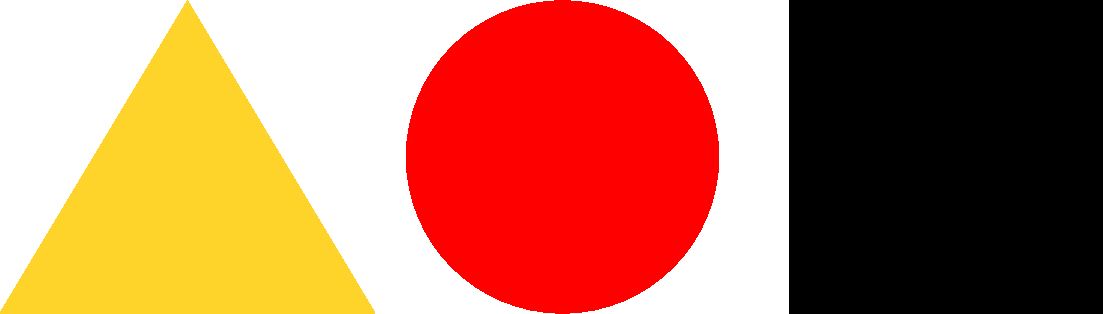
\includegraphics[scale = 0.2]{pictures/schad2.pdf}
\end{center}

\begin{center}
What topologist sees: \includegraphics[scale = 0.2]{pictures/schad3.pdf}
\end{center}

\end{frame}

\begin{frame}{Homeomorphism}

\begin{block}{Definition}
Let $X$, $Y$ be topological spaces. $f\colon X\to Y$ is called a homeomorphism if
\begin{enumerate}
  \item $f$ is continuous;
  \item $f$ is a bijection;
  \item $f^{-1}$ is also continuous.
\end{enumerate}
If there exists a homeomorphism $f\colon X\to Y$, then $X$, $Y$ are called \textcolor{red}{homeomorphic spaces}. Notation $X\cong Y$.
\end{block}

\begin{center}
\includegraphics[scale = 0.2]{pictures/schad1.pdf}
\end{center}

\pause

Example: $(-1;1)\cong \Ro$.

Example: Flat square is homeomorphic to flat circle.

Fact 1: $\cong$ acts like equivalence relation: if $X\cong Y$ and $Y\cong Z$, then $X\cong Z$.

Fact 2: if $X\cong Y$ and $X$ is compact, then $Y$ is compact.

\end{frame}

\begin{frame}{Coffee cup = donut}

\begin{center}
\begin{tabular}{M{2cm} M{1cm} M{1cm}}
  \includegraphics[scale = 0.4]{pictures/TorusMug/9ad666e1dab24639823928c242b3bdf0xmTjuhH4RRvOJNiC-0.png} & $\cong$ & \includegraphics[scale = 0.4]{pictures/TorusMug/9ad666e1dab24639823928c242b3bdf0xmTjuhH4RRvOJNiC-28.png} \\
\end{tabular}
\end{center}

\end{frame}

\begin{frame}{Also homeomorphic, but do not continuously deform to each other}

\begin{center}
\includegraphics[scale = 0.4]{pictures/KnottedTorus.pdf}
\end{center}

\end{frame}

\begin{frame}{Invariants}

We want to distinguish non-homeomorphic shapes. Use \textbf{invariants} of homeomorphism.\pause

\begin{block}{The fundamental invariant in topology}
Number of connected components. The set of connected components of $X$ is denoted $\pi_0(X)$.
\end{block}

Fact: $X\cong Y$ implies $X,Y$ have the same number of connected components.\pause

But we have:

\begin{center}
\begin{tabular}{M{1cm} M{1cm} M{1cm} M{1cm} M{1cm} M{1cm} M{1cm}}
  \includegraphics[scale = 0.15]{pictures/sphere.png} & $\ncong$ & \includegraphics[scale = 1]{pictures/torus.png}
  & $\ncong$ & \includegraphics[scale = 1]{pictures/krendel.png} & $\ncong$ & \includegraphics[scale = 1]{pictures/3krendel.png}
\end{tabular}
\end{center}

We need more invariants to distinguish them.

\end{frame}


\begin{frame}{Ideas of invariants}

\begin{itemize}
  \item Naive invariants motivated by connectivity \pause
  \item Internal dimension \pause
  \item Number of holes, fundamental group \pause
  \item Local properties \pause
  \item Orientability \pause
  \item Universal constructions $X\mapsto \mathcal{F}(X)$ such that $X\cong Y$ implies $\mathcal{F}(X)\cong \mathcal{F}(Y)$
\end{itemize}

\end{frame}

\begin{frame}{Homotopy between maps}

\begin{block}{Equivalence of maps}
Continuous maps $f,g\colon X\to Y$ are called \textcolor{red}{homotopy equivalent}, if one can be continuously deformed to another. Formally $f\sim g$ iff there exists a continuous map $F\colon X\times [0,1]\to Y$ such that $F(x,0)=f(x)$ and $F(x,1)=g(x)$.
\end{block}

Symbol $f\simeq g$. \pause

Facts: 
\begin{itemize}
  \item Homotopy equivalence is equivalence.
  \item Homotopy is path in the space $Y^X=\Maps(X,Y)$ of continuous maps from $X$ to $Y$ between $f$ and $g$.
\end{itemize}

\end{frame}



\begin{frame}{Homotopy equivalent spaces}

\begin{block}{Homotopy equivalence of spaces}
Two topological spaces $X,Y$ are called \textcolor{red}{homotopy equivalent}, if there exist continuous maps $h\colon X\to Y$ and $k\colon Y\to X$, such that $h\circ k\simeq \id_Y$ and $k\circ h\simeq \id_X$.
\end{block}

Symbol $X\simeq Y$. \pause Informally: two spaces are homotopy equivalent iff one is obtained from another by thinning and thickening.\pause

A space $X$ is called \textcolor{red}{contractible} if $X\simeq\pt$ ($\pt$ is a 1-point space).\pause

Facts:
\begin{itemize}
  \item Homotopy equivalence is an equivalence.
  \item Convex sets of $\Ro^n$ are contractible.
  \item A graph (its picture) is contractible iff it is a tree.
\end{itemize}

\end{frame}

\begin{frame}{Homotopy equivalence: some pictures}

\begin{center}
\includegraphics[scale = 0.6]{pictures/Homotopy.pdf}
\end{center}

We allow to make objects thin and thick.

\end{frame}


\begin{frame}{Contractible spaces}

\begin{center}
\includegraphics[scale = 0.3]{pictures/contractible.pdf}
\end{center}

Bing's house is an example of a contractible space which cannot be contracted to a point in a tree-like manner. 

\end{frame}



\begin{frame}{Homotopy invariants}

Invariants of homotopy equivalence:

\begin{itemize}
  \item Number of connected components \pause
  \item Fundamental group $\pi_1(X)$  \pause
  \item Homology vector spaces and Betti numbers (to be discussed)\pause
\end{itemize}

Not invariants:

\begin{itemize}
  \item Dimension \pause
  \item Local things \pause
  \item Orientability 
\end{itemize}

\end{frame}

\begin{frame}{Constructivity}

\begin{center}
\textcolor{red}{How can we explain shapes to computer?} \pause
\end{center}

Basically:
\begin{enumerate}
  \item Formulas (and their geometrical interpretations)
  \item Discrete data structures (and their topological interpretations)
\end{enumerate}

such as graphs, simplicial complexes, partially ordered sets, etc.


\end{frame}

\begin{frame}{Simplicial complex}


\begin{center}
\includegraphics[scale=0.3]{pictures/simpcomp.pdf}
\end{center}

\end{frame}

\begin{frame}{Simplicial complex}

\begin{block}{Definition}
\textcolor{red}{Simplicial complex} on a finite vertex set $V$ is a collection $K\subset 2^V$ satisfying the properties:
\begin{enumerate}
\item if $I\in K$ and $J\subset I$, then $J\in K$;
\item $\varnothing\in K$. 
\end{enumerate}
Elements $I\in K$ are called simplices. If $|I|=k$, we say that $I$ is a $(k-1)$-dimensional simplex.
\end{block}

\begin{enumerate}
  \item Vertices $\{i\}$ --- simplices of dim $0$;
  \item Edges $\{i,j\}$ --- simplices of dim $1$;
  \item Triangles $\{i,j,k\}$ --- simplices of dim $2$;
  \item etc.
\end{enumerate}

$\dim K$ is the maximal dimension of simplices of $K$.

\end{frame}

\begin{frame}{Geometrical realizations}

\begin{itemize}
  \item Graph is (a) a discrete object, (b) a picture.
  \item Some graphs cannot be drawn in $\Ro^2$ without self-intersections.
  \item But all graphs can be drawn in $\Ro^3$
\end{itemize}\pause
Similarly:
\begin{itemize}
  \item Simplicial complex $K$ is a discrete object.\pause
  \item In order to understand it as a continuous topological space, some picture in $\Ro^d$ should be drawn. It is called \textbf{the geometrical realization} of $K$ and denoted $|K|$.\pause
  \item It is easy to draw simplicial complex in the space of dimension $d=|V|$.
\end{itemize}

\textbf{Fact:} simplicial complex of dim $k$ can be drawn in $\Ro^{2k+1}$ without self-intersections.

\end{frame}

\begin{frame}{Geometrical realizations}

Simplicial complex is a discrete structure and can be encoded in computer. But in general:

\begin{itemize}
  \item There is no algorithm to check $|K|\cong |L|$ given $K$ and $L$.
  \item There is no algorithm to check $|K|\simeq |L|$ given $K$ and $L$.
  \item There is no even an algorithm to check $|K|\simeq\pt$ given $K$!
\end{itemize}

1-dimensional simplicial complexes (aka graphs) are simpler:
\begin{itemize}
  \item Homeomorphism of two graphs can be checked algorithmically.
  \item Homotopy equivalence of two graphs can be checked algorithmically.
\end{itemize}

\end{frame}




\begin{frame}{1-skeleton}

\begin{center}
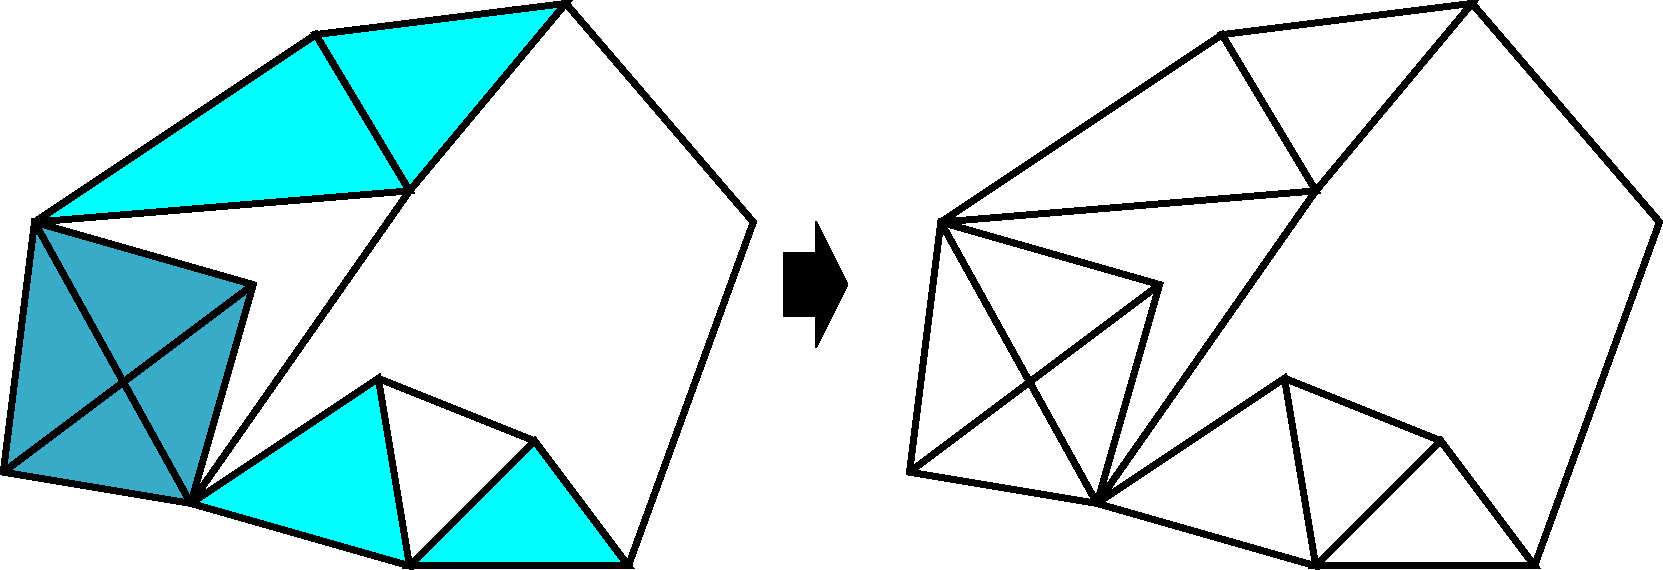
\includegraphics[scale=0.3]{pictures/skeleton.pdf}
\end{center}

\end{frame}

\begin{frame}{Clique complex}

\begin{center}
\includegraphics[scale=0.3]{pictures/clique.pdf}
\end{center}

*Clique = subgraph isomorphic to full graph.

\end{frame}

\begin{frame}{Clique complex}

Clique complex makes it possible to transform a graph into a high-dimensional structure. 

Since graphs are everywhere, this observation opens a way to use topological invariants everywhere.   

\end{frame}
%
%\begin{frame}{A principal incompatibility between ``topology'' and ``applied''.}
%
%\begin{itemize}
%  \item Data analysis and machine learning deal with real numbers and real optimization.
%  \item Topological invariants are discrete. There is no space with $2.3457$ many connected components or $\frac{5}{6}$ many holes.
%  \item How can we make Topology ``applied''?
%\end{itemize}
%\pause
%
%\begin{block}{Introduce ``topological processes''!}
%Let $X_t$ be a space depending on time $t\in\Ro$. If $t_1\leq t_2$, we assume there is a map
%\[
%f_{t_1\leqslant t_2}\colon X_{t_1}\to X_{t_2},
%\]
%such that $f_{t\leqslant t}=\id_{X_t}$ and $f_{t_2\leqslant t_3}\circ f_{t_1\leqslant t_2}=f_{t_1\leqslant t_3}$.
%\end{block}
%
%\end{frame}
%
%\begin{frame}{Esoteric formula}
%
%\[
%\dfrac{\mbox{Applied topology}}{\mbox{Topology}}=\dfrac{\mbox{Stochastic processes}}{\mbox{Probability theory}}=\mbox{Time!}
%\]
%
%\end{frame}
%
%\begin{frame}{Idea of applied topology}
%
%\begin{block}{Topological process}
%Let $X_t$ be a space depending on time $t\in\Ro$ and there are maps $f_{t_1\leqslant t_2}\colon X_{t_1}\to X_{t_2}$.
%\end{block}
%
%Usually, all connecting maps $f_{t_1\leqslant t_2}$ are inclusions. In this case the process is called a \textbf{filtration}.
%
%\begin{block}{Idea}
%\begin{itemize}
%  \item We may average topological invariants along all values of time $t$.
%  \item This gives real-valued invariants which can be optimized using methods of machine learning.
%\end{itemize}
%\end{block}
%
%\end{frame}
%
%\begin{frame}{Important construction}
%
%\begin{block}{Sublevel set filtration}
%Let $f\colon \Ro^d\to \Ro$ be a function. Consider sublevel sets of $f$
%\[
%X^f_t=\{x\in \Ro^d\mid f(x)\leqslant t\}
%\]
%This is a filtration.
%\end{block}
%
%\begin{center}
%  \includegraphics[scale = 0.13]{pictures/sublevel.pdf}
%\end{center}
%
%\end{frame}
%
%\begin{frame}{Another important construction}
%
%\begin{block}{\v{C}ech filtration}
%Let $X=\{x_1,\ldots,x_m\}\subset \Ro^d$ be a finite set (point cloud). Itself, the space $X$ is not interesting topologically. But we may surround each point with a ball of variable radius $t/2$, and see how topology evolve:
%\[
%X_t=\bigcup_{i=1}^m B_{t/2}(x_i)
%\]
%This is a filtration defined for $t\geqslant 0$.
%\end{block}
%
%\end{frame}
%
%\begin{frame}{\v{C}ech filtration}
%
%\begin{center}
%  \includegraphics[scale = 0.14]{pictures/sampling.pdf}
%\end{center}
%
%\end{frame}
%
%\begin{frame}{Toy example: average number of components}
%
%Let $X=\{x_1,\ldots,x_m\}\subset \Ro^d$ be a point cloud and $X_t$ its \v{C}ech filtration. Let $\nc(X_t)$ be the number of connected components of $X_t$.
%
%\begin{block}{A new invariant}
%Define the number
%\[
%\overline{\nc}(X)=\int_{0}^{+\infty} (\nc(X_t)-1)dt.
%\]
%\end{block}
%\pause
%
%Question: any guess what $\overline{\nc}(X)$ is?
%
%\begin{center}
%Demonstration: \href{https://play.unity.com/mg/other/builds-4z-1}{press to play in browser}
%\end{center}
%
%\end{frame}
%
%\begin{frame}{Toy example: evolution of components}
%
%\begin{block}{Answer:}
%$\overline{\nc}(X)$ equals the length of the minimal spanning tree of $X$. Guess why.
%\end{block}
%
%\pause
%
%\begin{center}
%  Dendrogram \includegraphics[scale = 0.3]{pictures/dendrogram.pdf}
%\end{center}
%
%Remark: nobody knows how to encode such dendrograms.
%
%\end{frame}
%
%\begin{frame}{Persistent homology}
%
%\begin{block}{Homology}
%Homology = higher dimensional analogue of counting connected components. Persistent homology = evolution of homology in time.
%\end{block}
%
%My plan for next lectures:
%
%\begin{enumerate}
%  \item Define the notion of simplicial complex.
%  \item Define cycles and homology in simplicial complexes.
%  \item Define the notion of filtration of simplicial complexes.
%  \item Look how cycles evolve through filtration.
%  \item Barcodes.
%  \item Persistence diagrams.
%\end{enumerate}
%
%\end{frame}
%
%\begin{frame}{Today's lesson}
%
%My plan for the rest of this lecture and for the seminar: estimation of dimension.
%
%\textcolor{red}{Problem:} given a finite point-set $X\subset \Ro^d$, estimate its intrinsic dimension.
%
%\begin{enumerate}
%  \item Linear method: PCA.
%  \item \textbf{Nonlinear dimension estimation. }
%\end{enumerate}
%
%Approach: use length of minimal spanning tree (LMST).
%
%\end{frame}
%
%\begin{frame}{LMST for point clouds in $\Ro^d$}
%
%Assume that $x_i$, $i=1,\ldots,n$ are sampled independently from a continuous distribution on $k$-dimensional manifold $M^k\subset \Ro^d$.
%\begin{itemize}
%  \item $d$ : ambient dimension.
%  \item $k$ : intrinsic dimension.
%\end{itemize}
%
%\begin{block}{Theorem (Steele'88)}
%\[
%\LMST(A_n)\sim C_k n^{\frac{k-1}{k}}\mbox{ when } n\to\infty.
%\]
%\end{block}
%
%This gives a \textcolor{blue}{fractal-type} formula to estimate the \textcolor{red}{intrinsic dimension} from the point cloud:
%\[
%\dfrac{k-1}{k} = \beta = \lim_{n\to\infty}\dfrac{\log \LMST(A_n)}{\log n},
%\]
%hence $k=\dfrac{1}{1-\beta}$.
%\end{frame}
%
%
%\begin{frame}{Example}
%
%What is the intrinsic dimension in this case? PCA tells it is 2.
%
%\begin{center}
%  \includegraphics[scale = 0.5]{pictures/cloud1.pdf}
%\end{center}
%
%\end{frame}
%
%\begin{frame}{Example}
%
%What is the intrinsic dimension in this case? LMST tells it is closer to 0.
%
%\begin{center}
%  \includegraphics[scale = 0.5]{pictures/cloud2.pdf}
%\end{center}
%
%\end{frame}
%
%
%
%\begin{frame}{Erd\H{o}s--R\'{e}nyi metric graph}
%
%What if data are not chosen in $\Ro^n$ but rather take the form of a random metric graph?
%
%\begin{block}{Construction}
%Let us take $n$ points and set pairwise distances $d_{i,j}$ independently uniformly from $[0;1]$. Denote this \textcolor{red}{random metric graph} by $\Gamma_n$.
%\end{block}
%
%\begin{block}{General problem}
%What can we say about LMST of $\Gamma_n$?
%\end{block}
%
%%\href{https://colab.research.google.com/drive/146yQdZBsPGfYZwi1AGKJwSE5wjRwPnc1?usp=sharing}{Experiments}: sum of lifetimes of $\PH_0(K_t^{VR}(\Gamma_n))$ is around $1.2$ and does not grow with $n$.
%
%\end{frame}
%
%
%\begin{frame}{Experiments}
%
%\begin{center}
%  \includegraphics[scale = 0.5]{pictures/LMSTexperiment.png}
%\end{center}
%
%\[
%\mbox{\textcolor{purple}{Why this number is not growing?}}
%\]
%\pause
%\[
%\mbox{\textcolor{purple}{Do you recognize the number 1.2?}}
%\]
%\end{frame}
%
%
%\begin{frame}{Ap\^{e}ry's constant}
%
%\[
%\zeta(3)=\sum_{n=1}^{\infty}\dfrac{1}{n^3}\approx 1.20205
%\]
%
%\begin{block}{Theorem (Frieze'85)}
%Let $\LMST_n$ be the length of the MST for the random graph $\Gamma_n$.
%\begin{enumerate}
%  \item $\lim\limits_{n\to\infty} \Eo\LMST_n=\zeta(3)$;
%  \item $\lim\limits_{n\to\infty}P(|\LMST_n-\zeta(3)|>\varepsilon)=0$ for any $\varepsilon>0$.
%\end{enumerate}
%\end{block}
%
%\end{frame}
%
%\begin{frame}{Ideas for research}
%
%Choose any family of graphs $G_n$ with bounded diameter. For example, $G_n=K_{n,n}$. Define edge lengths independently at random.
%
%\begin{block}{Problem}
%What can you say about $\lim\limits_{n\to\infty} \LMST(G_n)$? If it is constant, then what is the constant? If it grows, then what is the asymptotics?
%\end{block}
%
%\end{frame}
%
%
%
%
%
%\begin{frame}{Sources}
%
%\begin{thebibliography}{12}
%
%\bibitem{CoHe} J.\,Costa, A.\,Hero, \textit{Manifold Learning with Geodesic Minimal Spanning Trees}, preprint \href{https://arxiv.org/abs/cs/0307038}{arXiv:cs/0307038}
%
%\bibitem{Frieze} A.\,M.\,Frieze, \textit{On the value of a random minimum spanning tree problem}, Discrete Applied
%Mathematics 10 (1985) 47--56.
%
%\bibitem{Hatcher} A.\,Hatcher, \textit{Algebraic topology}, Cambridge University Press, 2002.
%
%\bibitem{Steele}  J.\,M.\,Steele, \textit{Growth rates of Euclidean minimum spanning trees with power weighted edges}, The Annals of Probability, 16 (4): 1767–1787 (1988).
%
%\end{thebibliography}
%
%\end{frame}



\end{document}
